\qrchapter{https://forgottenpillar.com/rsc/sw-fp-chapter24}{Mustakabali wa Kanuni za Msingi}

Tayari tumesoma nukuu ifuatayo kutoka kwa sura “\textit{Msingi wa Imani yetu}”. Ni moja ya maono ya mbeleni ya Dada White ya matengenezo makubwa ambayo yangetokea miongoni mwa Waadventista Wasabato; mageuzi haya yangejumuisha kuacha Kanuni ya Msingi. Hivi ndivyo shirika jipya litakavyoanzishwa.

\egw{\textbf{Adui ya roho ametaka kuleta dhana kwamba matengenezo makubwa yangetukia kati ya Waadventista Wasabato, na kwamba matengenezo haya yangefanyika \underline{yangejumuisha kuacha mafundisho ambayo yanasimama kama nguzo za imani yetu} na kuhusika katika mchakato wa kujipanga upya}. Je, matengenezo haya yangefanyika, matokeo yangekuwa nini? \textbf{Kanuni za ukweli ambazo Mungu katika hekima yake ametoa kwa kanisa la masalio zingetupwa. Dini yetu ingebadilishwa. \underline{Kanuni za msingi ambazo zimeendeleza kazi kwa miaka hamsini iliyopita ingehesabiwa kama makosa}}. \textbf{Shirika mpya lingeanzishwa. Vitabu vya namna mpya vingeandikwa. Mfumo wa falsafa ya kiakili ingeanzishwa}. Waanzilishi wa mfumo huu wangeenda katika miji na kufanya kazi ya ajabu. Sabato, bila shaka, ingechukuliwa kuwa nyepesi, kama vile Mungu aliyeiumba. Hakuna kitu kingeruhusiwa kusimama katika njia ya harakati mpya. Viongozi wange-fundisha kwamba wema ni bora kuliko uovu; lakini \textbf{Mungu akiondolewa}, wangeweka \textbf{utegemezi wao kwa nguvu za kibinadamu}, ambazo, bila Mungu, hazina thamani. Msingi wao ungejengwa juu ya mchanga, na dhoruba na tufani zingefagilia mbali muundo.}[Lt242-1903.13; 1903][https://egwwritings.org/read?panels=p7767.20]

\egwnogap{Nani mwenye mamlaka ya kuanzisha harakati hizo? \textbf{Tuna Biblia zetu. Tuna uzoefu wetu, unaothibitishwa na utendaji wa kimiujiza wa Roho Mtakatifu}. \textbf{Tuna ukweli ambao haukubali kufifiwa au kubati-lishwa.} \textbf{\underline{Je, hatutakataa kila kitu ambacho hakipatani na ukweli huu}?}}[Lt242-1903.14; 1903][https://egwwritings.org/read?panels=p7767.21]

Ellen White saw the effort of the enemy to remove these \emcap{Fundamental Principles}. They have sustained the work from the beginning. They were truths attested by the miraculous working of the Holy Spirit, and they admit no compromise. \egwinline{Shall we not repudiate everything that is not in harmony with this truth?}

Ellen White aliona juhudi za adui kuondoa \emcap{Kanuni za Msingi} ambazo zimedumisha kazi tangu mwanzoni. Zilikuwa kweli zilizothibitishwa na kazi ya kimiujiza ya Roho Mtakatifu, na hazikubali maafikiano. \egwinline{Je, hatutakataa kila kitu kilichopo ambacho haipatani na ukweli huu?}

\begin{figure}
    \centering
    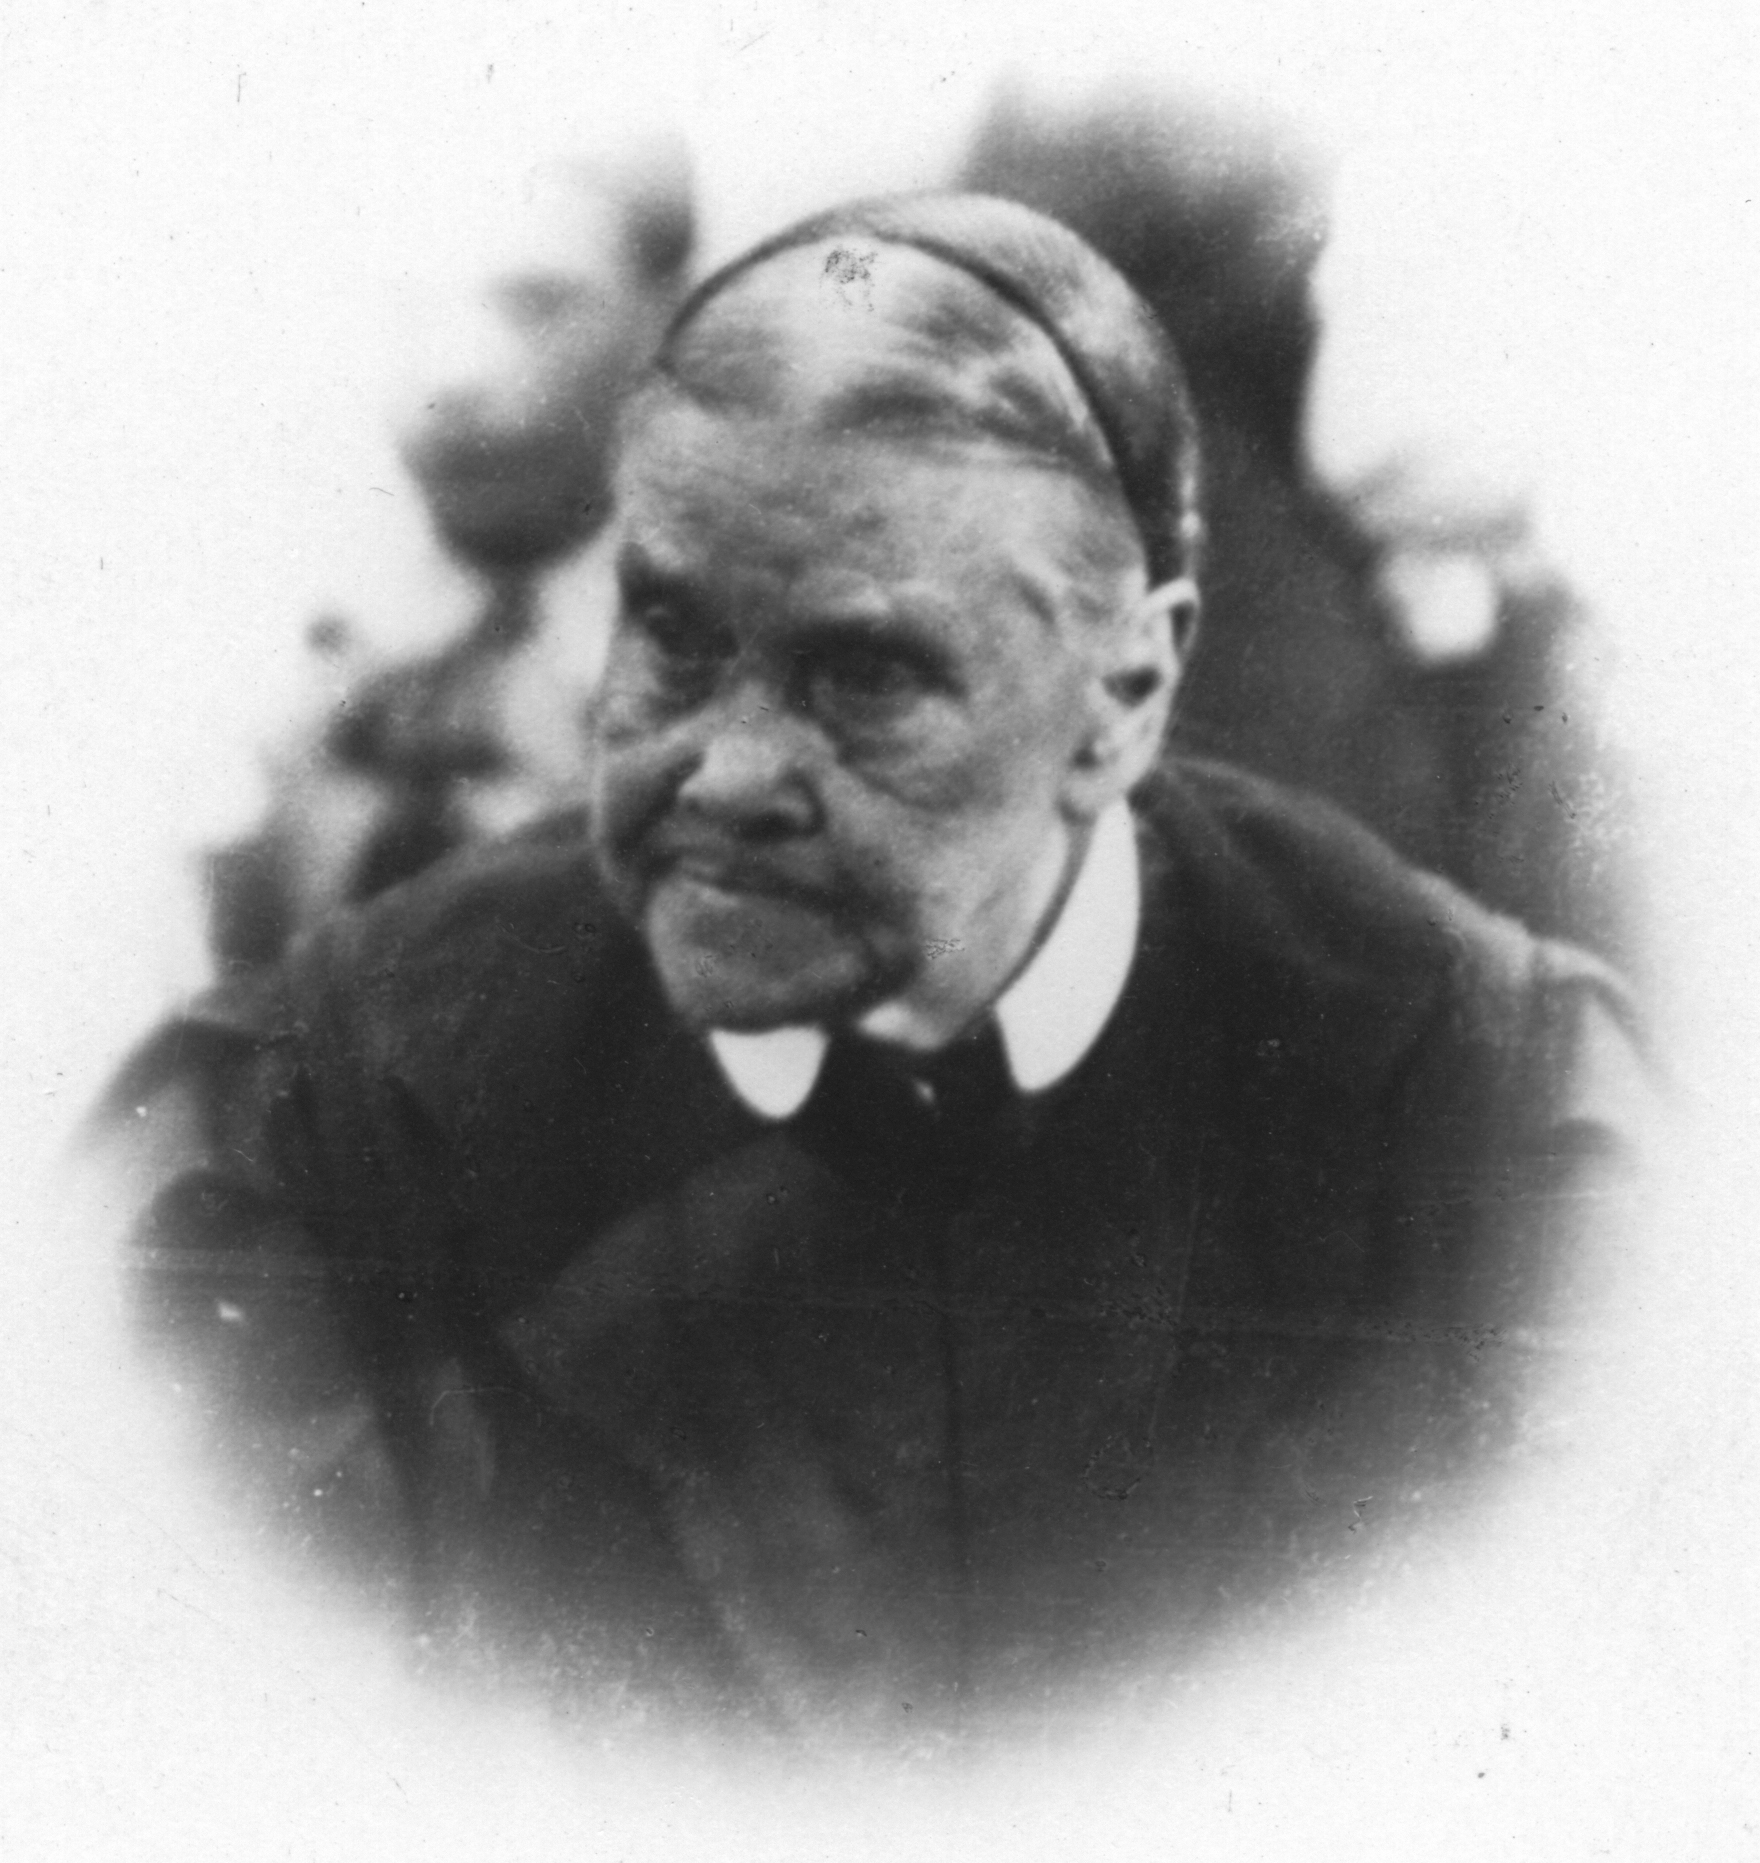
\includegraphics[width=1\linewidth]{images/ellen-white-1913.jpg}
    \caption*{Ellen G. White, 1913}
    \label{fig:e-white-1913}
\end{figure}

Dada White alitutabiria wakati ujao. Tunatazama utimilifu wake leo. Kulinganisha  \emcap{Kanuni za Msingi} na Imani za Msingi za leo, tunaona kwamba dini yetu imebadilika. Imani yetu kuhusu \emcap{Umbile la Mungu} imebadilika. Vitabu vya agizo jipya vimeandikwa, ambvayo havina msingi wa Neno thabiti la Mungu. Mfumo wa falsafa ya kiakili imeanzishwa.

Matengenezo haya yalifanyika katika wakati wake. Hivi ndivyo alivyoeleza siku za Kanisa la Waadventista Wasabato katika wakati wake na katika siku zijazo:

\egw{Wakati huu ni wakati mzito na wa kutisha kwa kanisa. Malaika tayari wamejifunga mshipi, wakingoja agizo la Mungu la kumimina mabakuli yao ya ghadhabu ulimwenguni. Malaika wa kuangamiza wanachukua kazi ya kisasi, kwa maana Roho wa Mungu anajiondoa polepole kutoka kwa ulimwengu. Shetani pia anakusanya majeshi yake ya uovu, akiwaendea ‘wafalme wa dunia na wa ulimwengu mzima,’ kuwakusanya chini ya bendera yake, ili kuzoezwa kwa ajili ya ‘vita vya siku ile kuu ya Mungu Mweza Yote.’ \textbf{Shetani anapaswa kufanya jitihada zenye nguvu zaidi kwa ajili ya ustadi katika mzozo kuu wa mwisho. \underline{Kanuni za msingi zitatolewa, na maamuzi yatafanywa kuhusiana nazo}. Mashaka yanatawala kila mahali}. Kutomcha Mungu kunazidi. \textbf{Imani ya washiriki binafsi wa kanisa itajaribiwa kana kwamba hakuna mtu mwingine duniani}...}[Ms1a-1890.8; 1890][https://egwwritings.org/read?panels=p6780.13]

Juhudi zenye nguvu zaidi za Shetani ni kuondoa \emcap{Kanuni za Msingi} kwa kuzifunika mashaka ndani. Kwa kuzingatia mtazamo wa leo tunashuhudia ukweli wa unabii wa Ellen White .

\egw{Nawaambia sasa, ya kwamba nitakapolazwa, \textbf{mabadiliko makubwa yatatokea}.}[Ms1-1915.2; 1915][https://egwwritings.org/read?panels=p10771.9]

Swali la kweli tunalo sisi wenyewe ni, wakati \emcap{Kanuni za Msingi} zinapokuwa zikitolewa, nitafanya uamuzi gani juu yao? Je, hatutakataa kila kitu ambacho hakipatani na kanuni hizi? Utafanya uamuzi gani?

% The future of the Fundamental Principles

\begin{titledpoem}
    \stanza{
        In the early whisper of prophecy’s sound, \\
        Ellen White warned where dangers abound. \\
        "The enemy plots," she sternly declared, \\
        "To dismantle truths our forebears shared."
    }

    \stanza{
        Fundamental Principles, strong and sure, \\
        Once the bedrock, pure and unpure. \\
        Now the sands shift beneath our creed, \\
        Where new doctrines grow like wayward weed.
    }

    \stanza{
        Reformation masked as light so bright, \\
        Undermines the pillars, eroding right. \\
        Books rewritten, philosophies anew, \\
        Skepticism veils what once we knew.
    }

    \stanza{
        Shall the Sabbath lose its sacred glow? \\
        Shall we forget the God that we owe? \\
        "The foundation crumbles," so it seems, \\
        As truth is lost to intellectual dreams.
    }

    \stanza{
        Look back to the days, to the Spirit-led start, \\
        Where divine truths were etched in heart. \\
        Satan’s strategies, cunning and keen— \\
        Eroding what once was clearly seen.
    }

    \stanza{
        So, brethren, now to the past return, \\
        To the roots of faith, let our hearts yearn. \\
        For the warnings spoken, the visions seen, \\
        Call us to defend what they truly mean.
    }

    \stanza{
        Stand firm in the storm as the tempests roar, \\
        Reclaim the truths worth fighting for. \\
        Ellen’s voice echoes, stark and clear: \\
        "Repudiate the false, hold the righteous near."
    }

    \stanza{
        Make your choice, as the battle lines draw, \\
        On the side of the timeless, divine law. \\
        To the Fundamental Principles, fiercely hold, \\
        The original faith, courageous and bold.
    }
\end{titledpoem}
